
% 背景介绍
\section{绪论}
% 
\subsection{研究背景与意义}
\begin{frame}{研究背景与意义}
\begin{figure}[htp]
    \centering
    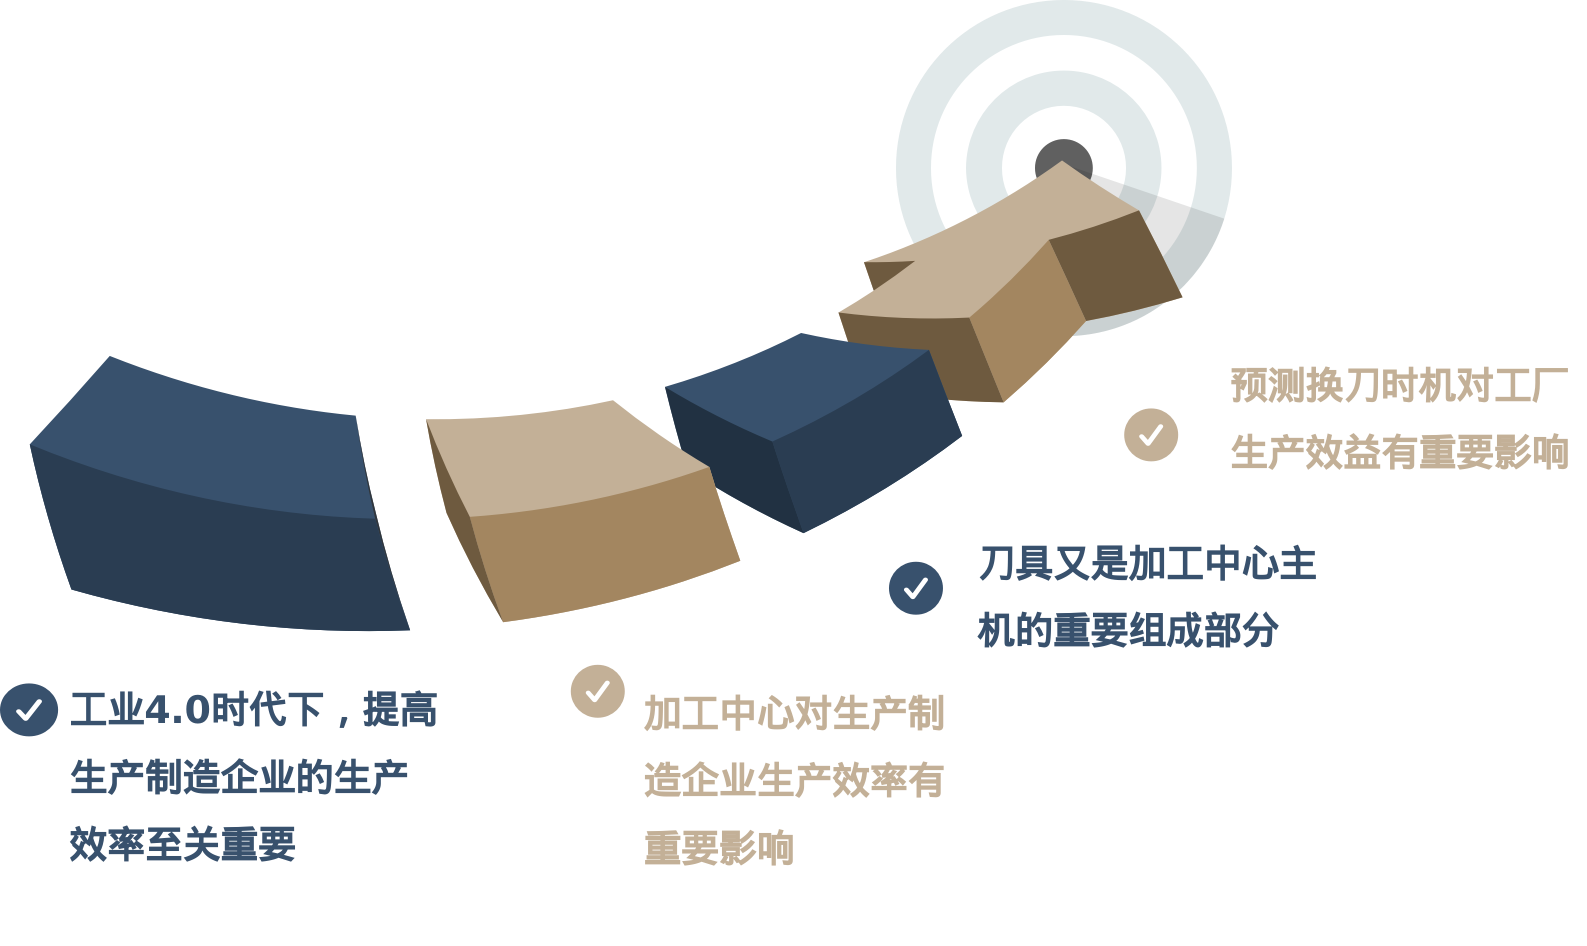
\includegraphics[width=10cm]{绪论/研究背景.png}
    % \caption{研究背景}
\end{figure}
% \ \ \ \ \ 针对真实数控机床铣削刀具磨损过程数据,进行特征工程处理后转化为对目标刀具磨损量敏感的特征值,为后者处理机床数据提供一定的参考意义。在此基础上,建立反向传播神经网络刀具磨损量预测模型,有利于选择最优换刀时间,提高生产效率,节约生产成本,提升我国制造业产业加工质量。
\ \ \ \ \ \ 我们使用反向传播神经网络与边缘计算这两种革命性的技术,替代传统的刀具退化测量模型,在机床不停机的情况下也可以实时获取刀具磨损量。当刀具磨损量到达阈值时,系统会作出警报,提醒工人及时更换刀具。\par
\end{frame}
% 
% 
% \subsection{研究意义}
% \begin{frame}{研究意义}

% \end{frame} 
\subsection{方案总体研究框架}
\begin{frame}{方案总体研究框架}
% 
\begin{figure}[htp]
    \centering
    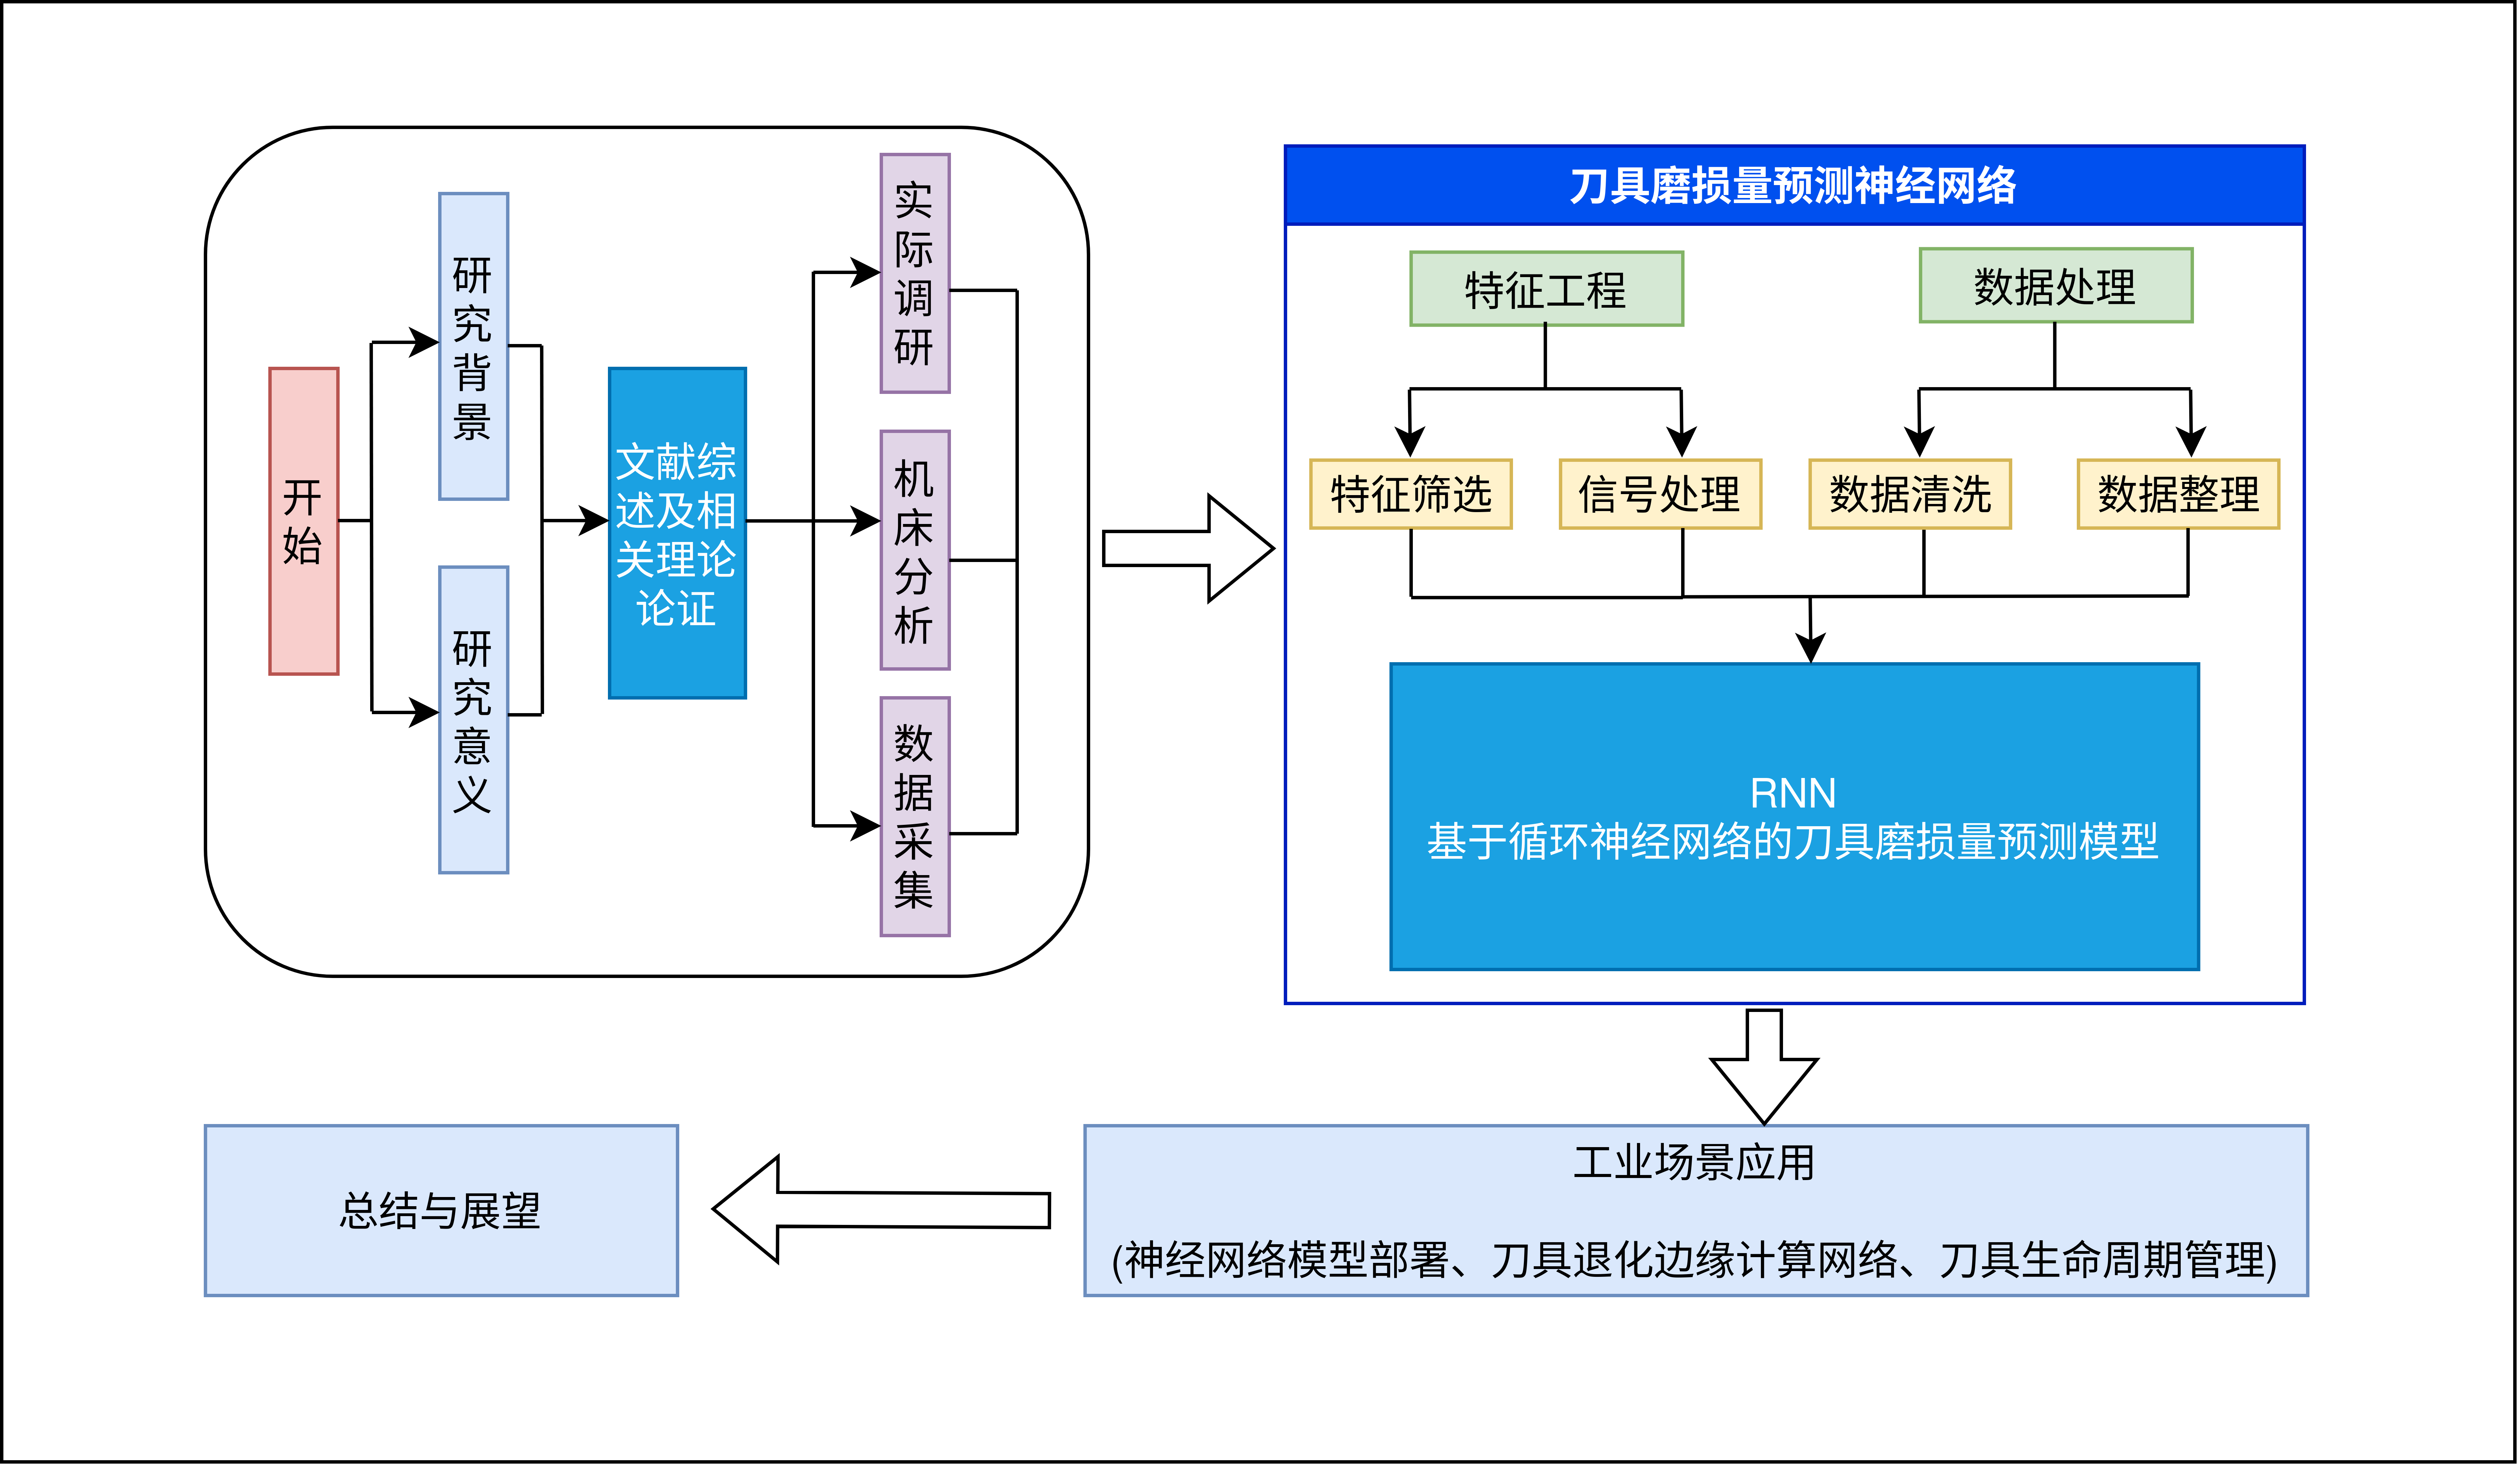
\includegraphics[width=12cm]{绪论/OpenIE研究架构.png}
    \caption{方案总体研究框架}
\end{figure}
% 
% 
\end{frame} 
% 
\subsection{传统刀具磨损量测定存在的问题与仿真实验}
\begin{frame}{传统刀具磨损量测定存在的问题(物理仿真实验)}
\begin{figure}[htp]
    \centering
    \includegraphics[width=12cm]{绪论/traditionproblem.png}
    % \caption{刀具磨损预测流程图}
\end{figure}
\ \ \ \ \ \ 为对比深度学习预测刀具退化程度与传统测定方法优劣,我们使用FlexSim进行制造系统仿真,传统方法测定刀具退化由于需要缓冲时间进行停机检查,且考虑到高级工程师工资,次品率等因素。深度学习法单位时间产能提升18.5\%,成本降低1成,次品率降低6.7\%。\par
\end{frame} 
% 
